\section{Text Editor using Qt}
This text editor is made using Qt. Qt is the C++ framework. It has most used features that a text editor have. 
\noindent As my 6 weeks training project,  I worked  in Qt creater and made a text editor.
Qt Creator is a complete IDE for creating applications with Qt Quick and the Qt application framework.
\begin{figure}[h]
\begin{center}
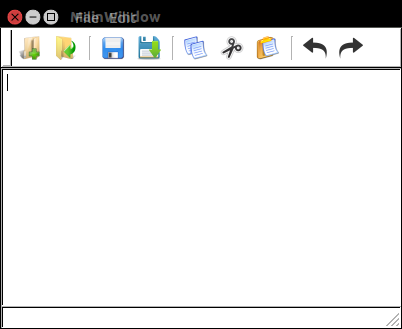
\includegraphics[scale=0.7]{images/dp/qpad.png}
\caption{qPad- The Text Editor}
\end{center}
\end{figure}

It has the following features:
\begin{itemize}
\item New File
\item Open File
\item Save File
\item Save as File
\item Copy
\item Paste
\item Cut
\item Undo
\item Redo
\end{itemize}

%Qt  is  designed  for  developing  applications  and  user  interfaces  once  and  deploying  them  across  several
%desktop and mobile operating systems. 
In this text editor we can make new text file and edit text. We can copy, cut and paste text easily. We can save and our text document in any location and open text document from any location. 

\subsection{Installation Guide}
To install qPad, you need to clone it from github.
\begin{itemize}
\item Go to terminal and type\\\\
\textit{git clone http://www.github.com/darshpreets/Text-editor.git}
\item Now go to the directory qpad by using: \\\\
\textit{cd qPad}
\item Now running qmake command: \\\\
\textit{qmake qpad.pro}
\item Now MakeFile will be generated. After that run make: \\\\
\textit{make}
\item An executable file will be generated. Execute it using: \\\\
\textit{./qpad}
\end{itemize}